%
% 5-fourier.tex
%
% (c) 2023 Prof Dr Andreas Müller
%
\section{Fourier-Transformation
\label{buch:gruppen:section:fourier}}
In diesem Abschnitt soll die Gruppe $\mathbb{R}$ etwas genauer untersucht
werden.
Das Skalarprodukt für Funktionen auf dieser Gruppe ist eine Integral über
einen unendlichen Definitionsbereich, so entsteht das Problem, dass
selbst beschränkte Funktionen ein unendliches Skalarprodukt haben können.
Wir müssen uns daher auf Funktionen beschränken, die nur auf einer
kompakten Teilmenge von $0$ verschieden sind und den Funktionenraum
daraus durch Vervollständigung aufbauen.

Im Gegensatz zur Gruppe der Winkel ist die Gruppe $\mathbb{R}$ nicht kompakt
und die Menge der Homomorphismen ist nicht diskret.
Wir können also nicht mehr unendliche Summen verwenden, um eine Funktion
aus ihren Frequenzkomponenten zu synthetisieren.
Stattdessen müssen wir zu einem Integral übergehen.

%
% Die Gruppe $G=\mathbb{R}$
%
\subsection{Die Gruppe $G=\mathbb{R}$
\label{buch:gruppen:fourier:subsection:gruppeR}}
Die duale Gruppe von $G=\mathbb{R}$ besteht aus den stetigen Homomorphismen
$\chi:\mathbb{R}\to\mathbb{C}^*$.
Solche Funktionen erfüllen die Funktionalgleichung $\chi(a+b)=\chi(a)\chi(b)$.

Ableitung der Funktionalgleichung nach $b$ an der Stelle $b=0$ führt auf
die Differentialgleichung
\[
\chi'(a) = \chi(a)\chi'(0),
\]
die Homomorphismen erfüllen also die Differentialgleichung
\[
\operatorname{const}
=
\frac{\chi'(x)}{\chi(x)} 
=
\frac{d}{dx}\log\chi(x)
\qquad\Rightarrow\qquad
\log\chi(x) = \operatorname{const}\cdot x
\qquad\Rightarrow\qquad
\chi(x) = e^{\alpha x}.
\]
Nur diejenigen Homomorphismen sind beschränkt und können dazu verwendet,
für die die Konstante $\alpha=ik$ imaginär ist, mit $k\in\mathbb{R}$.
Die duale Gruppe ist daher
\[
\hat{G}
=
\{
\chi\colon\mathbb{R}\to\mathbb{C}^*
\mid
\chi(x) = e^{ikx},\quad k\in \mathbb{R}
\}.
\]
Zu jedem Homomorphismus $\chi$ gehört also eine eindeutig bestimmte
Zahl $k\in\mathbb{R}$, die sogenannte {\em Wellenzahl},
\index{Wellenzahl}%
und umgekehrt.

Die Gruppe $G=\mathbb{R}$ ist abelsch, daher erwarten wir, dass 
$\hat{G}$ ebenfalls eine Gruppe ist.
Die Gruppenoperation entsteht nach
Abschnitt~\ref{buch:gruppen:gelfand:subsection:dual} aus der 
Multiplikation der Charaktere.
Seien also $\chi_1$ und $\chi_2$ zwei Homomorphismen
$\mathbb{R}\to\mathbb{C}^*$ und $k_1$ bzw.~$k_2$ die zugehörigen
Wellenzahlen in $\mathbb{R}$, es ist also
\[
\chi_1(x) = e^{ik_1x}
\qquad\text{und}\qquad
\chi_2(x) = e^{ik_2x}.
\]
Das Produkt
\[
\chi_1(x)\chi_2(x)
=
e^{ik_1x}e^{ik_2x}
=
e^{i(k_1+k_2)x}
\]
der beiden Charaktere ist wieder ein Homomorphismus
$\mathbb{R}\to\mathbb{C}^*$, der zur Wellenzahl $k_1+k_2$ gehört.
$\hat{\mathbb{R}}$ ist daher nicht nur als Menge das gleiche wie
die Menge der Wellenzahlen $k\in \mathbb{R}$, sondern auch als
Gruppe mit der Addition also Gruppenoperation.

Da für $\mathbb{R}$ das Lebesque-Mass translationsinvariant ist,
ist auch das Haar-Mass auf der dualen Gruppe $\hat{\mathbb{R}}=\mathbb{R}$
bis auf einen Normierungsfaktor bekannt.
Wir können ihn so wählen, dass die Transformations- und
Rücktransformationsformeln möglichst einfach werden.

%
% Fourier-Transformation
%
\subsection{Fourier-Transformation
\label{buch:gruppen:fourier:subsection:transformation}}
Im Abschnitt~\ref{buch:gruppen:fourier:subsection:dualR} wurde die
duale Gruppe von $G=\mathbb{R}$ bestimmt.
Nach der allgemeinen Theorie der Gelfand-Transformation sind die
Werte der Gelfand-Transformation auf Funktionen mit kompaktem
Träger die Skalarprodukt
\begin{equation}
(\mathscr{G}f)(\chi)
=
\langle \chi,f\rangle
=
\int_{\mathbb{R}} \overline{\chi(x)} f(x)\,dx
=
\int_{\mathbb{R}} e^{-ikx} f(x)\,dx,
\label{buch:gruppen:fourier:ft:integral}
\end{equation}
wenn $k$ die Wellenzahl des Charakteres $\chi(x)=e^{ikx}$ ist.
Das Integral~\eqref{buch:gruppen:fourier:ft:integral} ist nicht nur
für Funktionen mit kompaktem Träger definiert, sondern wegen $|\chi(x)|=1$
für beliebige integrierbare Funktionen.

\begin{definition}[Fourier-Transformation auf $\mathbb{R}$]
Die Fourier-Transformation einer integrierbaren Funktion $f\in L^1(\mathbb{R})$
\index{Fourier-Transformation!auf $\mathbb{R}$}%
ist die Funktion
\[
\mathscr{F}f
\colon
k\mapsto
(\mathscr{F}f)(k)
=
\hat{f}(k)
=
\int_{\mathbb{R}} e^{-ikx}f(x)\,dx.
\]
\end{definition}

%
% Unschärfe-Relation
%
\subsection{Unschärferelation
\label{buch:gruppen:fourier:subsection:unschaerfe}}
Musiker haben die Erfahrung gemacht, dass es schwierig ist, die
Tonhöhe eines kurzen Tones festzustellen.
Die Genauigkeit der Frequenzbestimmung wächst, wenn die Dauer des
analysierten Signals länger wird.
Da das Signal und sein zugehöriges Frequenzspektrum über die
Fourier-Transformation miteinander verbunden sind, suggeriert dies,
dass ein Signal, das in der Zeit wie ein kurzer Ton gut lokalisiert ist,
im Frequenzbereich schlecht lokalisiert ist.
Umgekehrt erreicht man gute Lokalisierung und damit genaue Tonhöhenbestimmung
im Frequenzbereich, wenn das Signal zeitlich nicht klar bestimmt ist.
Die in diesem Abschnitt entwickelte Unschärferelation fasst diesen intuiven
mathematisch präzis.

In Abschnitt~\ref{buch:diskret:section:unschaerfe} wird gezeigt, dass
Unschärferelationen eine sehr allgemeine Eigenschaft der Transformationen
sind, denen man in der harmonischen Analysis begegnet.

%
% Dirac-delta-Funktion
%
\subsubsection{Dirac-\textdelta-Funktion}
In der elementaren Theorie der Fourier-Transformation wird oft 
die ``Dirac-\textdelta-Funktion'' $\delta(x)$ eingeführt, die die
Eigenschaft haben soll, dass
\begin{equation}
\int_{-\infty}^\infty \delta(x) f(x)\,dx = f(0)
\label{buch:gruppen:fourier:eqn:deltadef}
\end{equation}
haben soll.
Eine solche Funktion im üblichen Sinne kann es natürlich nicht geben.
Da das Integral nicht von den Werten $f(x)$ mit $x\ne 0$ abhängen darf,
muss $\delta(x)=0$ sind für $x\ne 0$.
Damit kann das Integral nur vom Funktionswert $\delta(0)$ abhängen,
einzelne Werte eines Integrals können aber ein Integral nicht beeinflussen.

Es kann also eine Delta-Funktion nicht geben, aber die Folge von
glatten Funktionen
\[
d_n(x) = \frac{1}{\sqrt{2\pi n}} e^{-x^2/n}
\]
ist eine gute Approximation dafür.
Die Funktionen $d_n$ sind ausserdem in $L^2(\mathbb{R})$ und
$L^2(\mathbb{R})$.
Tatsächlich konvergiert $\langle d_n,f\rangle \to f(0)$.
Dies ist nicht die einzige Möglichkeit, die Idee der 
Dirac-\textdelta-Funktion auf eine solide mathematische Basis zu
stellen.
Welche Vorgehensweise man auch immer wählt, sie produziert ein
mathematisches Objekt $\delta(x)$, welches man wie eine Funktion
mit der ``unmöglichen'' Eigenschaft
\eqref{buch:gruppen:fourier:eqn:deltadef}
behandeln kann.

Die Fourier-Transformierte der Dirac-\textdelta-Funktion ist
\[
(\mathscr{F}\delta)(k)
=
\int_{-\infty}\infty e^{-ikx}\delta(x)\,dx
=
e^{ik\cdot 0}
=
1.
\]
Für eine um $y$ verschobene Dirac-\textdelta-Funktion ist die
Fourier-Transformierte
\[
(\mathscr{F}T_y\delta)(k)
=
\int_{-\infty}^\infty e^{-ikx}\delta(x-y)\,dx
=
\int_{-\infty}^\infty e^{-ik(x'+y)}\delta(x')\,dx'
=
e^{-iky}.
\]
Die Fourier-Transformierte der Dirac-\textdelta-Funktion hat also 
konstant den Betrag $1$, sie ist nicht einmal integrierbar.

%
% Lokalisierung
%
\subsubsection{Lokalisierung}
Die Dirac-\textdelta-Funktion ist ein extremes Beispiel für eine
Funktion, die sehr präzise lokalisiert ist, ihr Träger besteht nur
aus einem einzigen Punkt.
Die Fourier-Transformation von $\delta(x)$ ist dagegen überhaupt
nicht lokalisiert, ganz im Gegenteil, $\mathscr{F}\delta$ hat für alle
Wellenzahlen den gleichen Wert.

Diese Eigenschaften kann man auch bei anderen Funktionen beobachten.
Zur Illustration wird im folgenden Beispiel auf einem Intervall
konstanten Funktion durchgerechnet.
Diese wird in der Signalverarbeitung auch als {\em Rechteckfenster}
\index{Rechteckfenster}
bezeichnet.

\begin{beispiel}
\label{buch:gruppen:fourier:beispiel:rechteck}
Die Funktion
\[
f_a(x)
=
\begin{cases}
\frac1{\sqrt{2a}}&\qquad -a\le x \le a\\
0&\qquad\text{sonst}.
\end{cases}
\]
ist integrierbar und quadratintegrierbar, es gilt
\[
\|f_a\|_2^2
=
\int_{-\infty}^\infty
|f_a(x)|^2
\,dx
=
\int_{-a}^a \frac{1}{2a} \,dx
=
1.
\]
Die Fouriertransformierte von $f_a$ ist
\begin{align*}
\mathscr{F}f_a
\colon k\mapsto
(\mathscr{F}f_a)(k)
&=
\int_{-\infty}^\infty e^{-ikx} f_a(x)\,dx
=
\frac{1}{\sqrt{2a}}
\int_{-a}^a e^{-ikx}\,dx
\\
&=
\frac{1}{\sqrt{2a}}
\biggl[
\frac{1}{-ik} e^{-ikx}
\biggr]_{-a}^a
=
\frac{1}{\sqrt{2a}}\biggl(
\frac{
e^{-ika}-e^{ika}
}{
-ik
}
\biggr)
\\
&=
\frac{2}{\sqrt{2a}k}\frac{e^{ika}-e^{-ika}}{2i}
=
\sqrt{\frac{2}{a}} \frac{\sin ka}{k}
=
\sqrt{2a} \frac{\sin ka}{ka}
=
\sqrt{2a}
\operatorname{si}(ka).
\end{align*}
Die Funktion
\[
\operatorname{si}(x)
=
\begin{cases}
1&\qquad \text{für $x = 0$}\\
\displaystyle\frac{\sin x}{x}&\qquad\text{sonst}
\end{cases}
\]
ist der nicht normierte Kardinalsinus.
Abbildung~\ref{buch:gruppen:fourier:fig:sinc} zeigt die Funktion 
$f_a$ und die Fourier-Trans\-for\-mier\-te $\mathscr{F}f_a$ für verschiedene
Werte von $a$.
\end{beispiel}

%
% sinc.tex
%
% (c) 2023 Prof Dr Andreas Müller
%
\begin{figure}
\centering
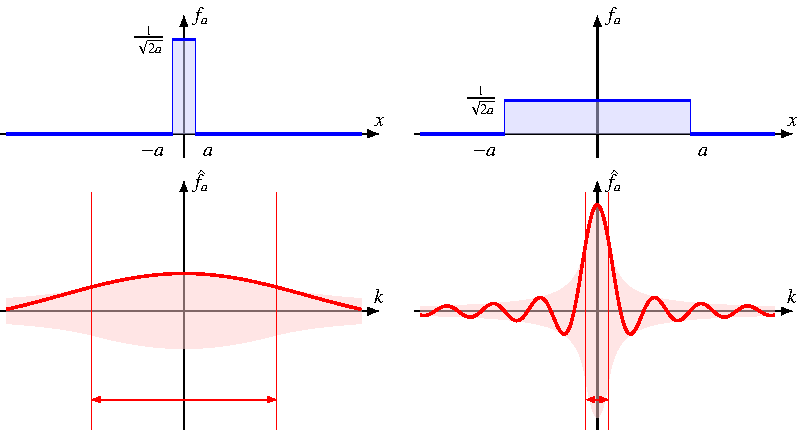
\includegraphics{chapters/030-gruppen/images/sinc.pdf}
\caption{Die Fourier-Transformierte der charakteristischen Funktion
eines Intervalls der Breite $2a$ ist skalierte Version des
Kardinalsinus.
\label{buch:gruppen:fourier:fig:sinc}}
\end{figure}


Die Abbildung~\ref{buch:gruppen:fourier:fig:sinc} zeigt auch, dass
die Fourier-Transformierte entlang der $k$-Achse gestaucht wird,
wenn die Funktion entlang der $x$-Achse gestreckt wird.
Dieses Resultat wird im folgenden Satz noch etwas präziser
formuliert.

\begin{satz}
\label{buch:gruppen:fourier:satz:FDa}
Sei $f\in L^1(\mathbb{R})$ eine integrierbare Funktion mit der
Fourier-Transformierten $\hat{f}=\mathscr{F}f$ und $D_af$ die um
den Faktor $a$ gedehnte Funktion $(D_af)(x)=f(ax)$, dann ist
die Fourier-Transformierte von $D_af$
\[
\widehat{D_af}(k)
=
\frac1a \hat{f}\biggl(\frac{k}{a}\biggr).
\]
\end{satz}

\begin{proof}[Beweis]
Wir berechnen die Fourier-Transformation
\begin{align*}
\widehat{D_af}(k)
&=
\int_{-\infty}^\infty
e^{ikx}D_af(x)
\,dx
\\
&=
\int_{-\infty}^\infty
e^{ikx}f(ax)
\,dx,
\intertext{indem wir die Substitution $ax=u$ und $dx = (1/a)\,du$ 
verwenden und damit}
&=
\frac{1}{a}
\int_{-\infty}^\infty
e^{i(k/a)u}f(u)
\,du
=
\frac{1}{a}
\hat{f}\biggl(\frac{k}{a}\biggr)
\end{align*}
erhalten.
\end{proof}

%
% Fourier-Transformation und Gauss-Verteilung
%
\subsubsection{Fourier-Transformation und Gauss-Verteilung}
Die Gauss-Verteilung spielt in der Wahrscheinlichkeitstheorie eine
spezielle Rolle, die ihr vom zentralen Grenzwertsatz zugewiesen wird.
Eine sehr grosse Summe vieler kleiner Einflüsse ist unabhängig von
der Verteilung der einzelnen Einflüsse im Wesentlichen normalverteilt.
Die Gauss-Verteilung hat aber auch in der Fourier-Theorie eine besondere
Bedeutung, wie die folgenden zwei Sätze zeigen.

\begin{satz}
\label{buch:gruppen:fourier:satz:gaussfourier}
Die Fourier-Transformierte der Gauss-Funktion $f(x)=e^{-ax^2}$ ist
\[
\hat{f}(k)
=
\sqrt{\frac{\pi}{a}}
e^{-k^2/2a},
\]
also wieder eine Gauss-Funktion.
\end{satz}

\begin{proof}
Wir berechnen die Fourier-Transformierte direkt aus
\begin{align*}
\hat{f}(k)
&=
\int_{-\infty}^\infty e^{-ikx} f(x)\,dx
=
\int_{-\infty}^\infty e^{-ax^2-ikx}\,dx.
\intertext{Durch quadratisches Ergänzen im Exponenten erhält man}
&=
\int_{-\infty}^\infty
e^{-ax^2-ikx+k^2/4a}
e^{-k^2/4a}
\,dx
= 
e^{-k^2/2a}
\int_{-\infty}^\infty
e^{-a(x-ik/2a)^2}
\,dx.
\intertext{Die Substitution $u=x-ik/2a$ mit $du=dx$ führt auf}
&=
e^{-k^2/4a}
\int_{-\infty}^\infty
e^{-au^2}
\,du
=
\sqrt{\frac{\pi}{a}}
e^{-k^2/4a}.
\end{align*}
Dieses formale Argument ist allerdings nicht ganz vollständig,
denn die Substitution $u=x-ik/2a$ ist eine Translation
in der komplexen Ebene.
Man kann aber mit den Methoden der komplexen Analysis zeigen, dass
sich das Integral durch die Verschiebung tatsächlich nicht ändert.
\end{proof}

Ein speziell interessanter Fall tritt auf, wenn $a=1/2a$ oder
$a^2=\frac14$ oder $a=\frac12$.
In diesem Fall ist die Fourier-Transformierte eine Vielfaches von
$e^{-k^2/2}$.

\begin{satz}[Gauss-Funktion als Eigenfunktion von $\mathscr{F}$]
\label{buch:gruppen:fourier:satz:gausseigen}
Die Funktion $f=e^{x^2/2}$ ist eine Eigenfunktion der Fouriertransformation
zum Eigenwert $\sqrt{2\pi}$, also
\[
\mathscr{F}f = \sqrt{2\pi} f.
\]
\end{satz}

%
% Die Heisenberg-Pauli-Weyl-Ungleichung
%
\subsubsection{Die Heisenberg-Pauli-Weyl-Ungleichung}
Um das in vorangegangenen Beispielen diskutierte Phänomen allgemein
zu fassen, dass eine gut lokalisierte Funktion eine schlecht lokalisierte
Fourier-Transformierte hat, benötigen wir ein Mass für die Lokalisierung.
Die Dirac-\textdelta-Funktion hat perfekte Lokalisierung, sie ist 
konzentriert auf ein Intervall der Länge $0$.
Ebenso sind die Funktionen $f_a$ auf einem Intervall der Länge $2a$
lokalisiert.
Die Länge des Trägerintervalls ist aber ein schlechtes Lokalisierungsmass,
denn der Träger aller Fourier-Transformierten $\mathscr{F}f_a$ ist,
Abbildung~\ref{buch:gruppen:fourier:fig:sinc} zeigt,
jeweils ganz $\mathbb{R}$.

Die in Abbildung~\ref{buch:gruppen:fourier:fig:sinc}
rot eigezeichnete Fourier-Transformierte von $f_a$ hat ihre grössten 
Werte in der Nähe von $k=0$.
Je grösser $a$ ist, desto besser sind die grossen Werte von $\mathscr{F}f_a$
in der Nähe von $k=0$ konzentriert.
Als Lokalisierungsmass könnte man eine Zahl verwenden, die die ``Breite''
des zentralen Buckels der Fourier-Transformierten misst.

Die Wahrscheinlichkeitsrechnung bietet ein besseres Mass für die
Lokalisierung an.
Mit geeigneter Normierung kann man man $|f(x)|^2$ als eine
Wahrscheinlichkeitsverteilung betrachten.
Die Varianz der Zufallsgrösse mit der Wahrscheinlichkeitsverteilung
$|f(x)|^2$ bietet sich als Lokalisierungsmass an.
Die Voraussetzung der Normierung kann immer erreicht werden, indem man
$f$ durch $f/\|f\|$ ersetzt.


\begin{definition}
Ist $f\in L^2(\mathbb{R}$ und $x|f(x)|^2$ integrierbar, dann sind
die Grössen
\begin{align*}
(\Delta x)^2
&=
\frac{1}{\|f\|^2}
\int_{-\infty}^\infty
(x-\langle x\rangle)^2
|f|^2(x)
\,dx
\\
(\Delta k)^2
&=
\frac{1}{\|\mathscr{F}f\|_2^2}
\int_{-\infty}^\infty
(k-\langle k\rangle)^2
|(\mathscr{F}f)(k)|^2
\,dk
\end{align*}
die Varianz einer Zufallsvariable mit Wahrscheinlichkeitsverteilung
$f^2/\|f\|_2^2$ bzw.~$\mathscr{F}f^2/\|\mathscr{F}f\|_2^2$.
\end{definition}

In der Wahrscheinlichkeitstheorie wird gezeigt, dass der Erwartungswert
$\langle x\rangle$ derjenige Wert der Konstanten $\mu$ in
\begin{equation*}
\frac{1}{\|f\|^2}
\int_{-\infty}^\infty
(x-\mu)^2 
|f(x)|^2
\,dx
\end{equation*}
ist, für den das Integral minimal wird.
Die Grösse $(\Delta x)^2$ ist als das Minimum der Grösse
\begin{equation}
\frac{1}{\|f\|_2^2}
\int_{-\infty}^\infty
(x-\mu)^2 
|f(x)|^2
\,dx
=
\frac{1}{\|f\|_2^2}
\int_{-\infty}^\infty
x^2\, |(T_{-\mu}f)(x)|^2
\,dx.
\label{buch:gruppen:fourier:eqn:translation}
\end{equation}
Da $(\Delta x)^2$ das Minimum des
Integrals~\eqref{buch:gruppen:fourier:eqn:translation} ist, wird
eine Abschätzung dieser Grösse immer auch für $(\Delta x)^2$ gelten.

Durch eine Translation wie $T_{-\mu}$ in
\eqref{buch:gruppen:fourier:eqn:translation}
ändert sich $\mathscr{F}f$ nur um einen Phasenfaktor,
der Erwartungswert und die Varianz von $k$ ändern sich nicht.
Und auch umgekehrt ändert eine Verschiebung der Fourier-Transformierten
$\mathscr{F}f$ entlang der $k$-Achse die Funktion $f$ nur um einen
Phasenfaktor, der sich auch $|f(x)|^2$ nicht auswirkt. 
Für die Beweis der folgenden Aussagen können wir daher wenn nötig annehmen,
dass $\langle x\rangle=0$ und $\langle k\rangle = 0$.

\begin{satz}[Heisenberg-Pauli-Weyl-Unschärferelation]
\label{buch:gruppen:fourier:satz:heisenberg-pauli-weyl}
Sind die Funktion $f(x)$, $xf(x)$ und $k(\mathscr{F}f)(k)$ alle in
$L^2(\mathbb{R})$ und $\lim_{x\to\pm\infty} \sqrt{x}|f(x)|=0$, dann
gilt
\begin{equation}
(\Delta x)^2
(\Delta k)^2
\ge 
\frac14.
\label{buch:gruppen:fourier:eqn:heisenberg-pauli-weyl}
\end{equation}
Gleichheit gilt genau für die Gauss-Funktionen $f(x)=Ce^{-ax^2}$, $a>0$.
\end{satz}

\begin{proof}[Beweis]
Wir schreben $F(k) = (\mathscr{F}f)(k)$ und möchten $(\Delta x)^2(\Delta k)^2$
nach unten abschätzen.
Nach der Bemerkung vor dem Satz dürfen wir davon ausgehen, dass die
Erwartungswerte $0$ sind.
Es genügt als  wie folgt zu rechnen:
\begin{align}
\|f\|_2^2
\|F\|_2^2
(\Delta x)^2
(\Delta k)^2
&=
\int_{-\infty}^\infty |x\,f(x)|^2\,dx
\int_{-\infty}^\infty |k\,F(k)|^2\,dk.
\notag
\intertext{Aus der Ableitungseigenschaft $ikF(k) = (\mathscr{F}f')(k)$
der Fourier-Transformation folgt}
&=
\int_{-\infty}^\infty |x\,f(x)|^2\,dx
\int_{-\infty}^\infty |(\mathscr{F}f')(k)|^2\,dk.
\notag
\intertext{Die Fourier-Transformation ändert die $L^2$-Norm nicht, es
folgt daher}
&=
\int_{-\infty}^\infty |x\,f(x)|^2\,dx
\int_{-\infty}^\infty |f'(x)|^2\,dx
=
\|xf(x)\|_2^2\cdot \|f'\|_2^2
.
\notag
\intertext{Nach der Cauchy-Schwarz-Ungleichung kann dieses Produkt
nach unten durch das Skalarprodukt}
&\ge
|\langle xf(x),f'(x)\rangle|
=
\biggl|
\int_{-\infty}^{\infty} xf(x)f'(x)\,dx
\biggr|^2
\label{buch:gruppen:fourier:eqn:cauchyschwarz}
\intertext{abgeschätzt werden.
Allerdings können beide Faktoren noch mit einem beliebigen Phasenfaktor
multipliziert werden oder die Faktoren können komplex konjugiert werden,
ohne dass sich der Wert ändert.
Wir wählen die Kombination}
&=
\biggl|
\int_{-\infty}^{\infty} xf(x)\overline{f'(x)}\,dx.
\biggr|
\notag
\intertext{Verwendet man nur den Realteil des Integranden, wird das Integral
noch kleiner, nämlich}
&\ge
\biggl|
\int_{-\infty}^{\infty} \Re(xf(x)\overline{f'(x)})\,dx
\biggr|^2
\label{buch:gruppen:fourier:eqn:realteil}
\\
&=
\biggl|
\int_{-\infty}^{\infty} \frac12\bigl(
xf(x)\overline{f'(x)}
+
\overline{ xf(x)\overline{f'(x)}}
\bigr)\,dx
\biggr|^2
\notag
\\
&=
\biggl|
\int_{-\infty}^{\infty}
\frac12x
\bigl(
f(x)\overline{f'(x)} + \overline{f(x)}f'(x)
\bigr)
\,dx
\biggr|^2
=
\biggl|
\int_{-\infty}^{\infty}
\frac12x
\frac{d}{dx}\bigl(f(x)\overline{f(x)}\bigr)
\,dx
\biggr|^2
\notag
\\
&=
\frac14 \biggl|
\int_{-\infty}^{\infty}
x\frac{d}{dx}(|f(x)|^2)
\biggr|^2
\notag
\intertext{Partielle Integration ergibt}
&=
\frac14
\biggl|
\biggl[
x|f(x)|^2
\biggr]_{-\infty}^\infty
-
\int_{-\infty}^{\infty}
|f(x)|^2
\,dx
\biggr|^2.
\notag
\intertext{Nach Voraussetzung verschwindet der erste Term.
Das Integral im zweiten Term ist das Quaddrat der $L^2$-Norm, also}
&=
\frac14\|f\|_2^4.
\notag
\intertext{Verfolgen wird die gesamte Ungleichungskette, finden wir}
\|f\|_2^2
\|F\|_2^2
(\Delta x)^2
(\Delta k)^2
&\ge 
\frac14
\|f\|_2^4.
\notag
\intertext{Verwendet man erneut, dass die Fourier-Transformation die $L^2$-Norm
nicht ändert, kann man die Normen wegkürzen und erhält schliesslich die
Ungleichung}
(\Delta x)^2
(\Delta k)^2
&\ge 
\frac14.
\notag
\end{align}
Damit ist die Ungleichung bewiesen, es bleibt noch zu zeigen, dass Gleichheit
nur für Gauss-Funktionen auftreten kann.
Gleichheit tritt auf, wenn in den Ungleichungen
\eqref{buch:gruppen:fourier:eqn:cauchyschwarz}
und
\eqref{buch:gruppen:fourier:eqn:realteil}
Gleichheit vorliegt.
Die zweite ist einfach: hier wird zum Realteil übergegangen, wenn sich
dabei nichts ändert, liegt Gleichheit vor, also genau für reelle Funktionen.
Die erste ist die Cauchy-Schwarz-Ungleichung, in der Gleichheit genau
dann vorliegt, wenn die Faktoren linear abhängig sind, wenn also
die Gleichung
\[
f'(x)
=
c
xf(x)
\]
gilt.
Die Differentialgleichung  lässt sich separieren:
\[
\frac{f'(x)}{f(x)} = \frac{d}{dx}\log f(x) = cx
\quad\Rightarrow\quad
\log f(x) = \frac12cx^2 + d
\quad\Rightarrow\quad
f(x) = Ce^{-ax^2},
\]
mit $-a = \frac12c$.
Die Konstante $a$ muss positiv sein, weil sonst $f(x)$ nicht
integrierbar ist.
Gleichheit tritt also genau auf für Gauss-Funktionen.
\end{proof}

%
% Unschärferelation inder Quantemechanik
%
\subsubsection{Unschärferelation in der Quantenmechanik}
In der Quantenmechanik wird der Zustand eines Teilchens durch die 
komplexwertige Wellenfunktion $\psi\colon\mathbb{R}^3\to\mathbb{C}$
beschrieben.
Die übliche Interpretation der Wellenfunktion ist, dass $|\psi(x)|^2$
die Wahrscheinlichkeitsdichte dafür ist, das Teilchen im Punkt $x$ zu
finden.
Der Erwartungswert der Position der des Teilchens bei einer Messung
ist daher
\[
\langle x\rangle
=
\int_{\mathbb{R}^3} x\, |\psi(x)|^2\,dx.
\]
Die erwartete Genauigkeit dieser Positionsbestimmung ist die Varianz
der Wahrscheinlichkeitsdichte des Ortes, also genau die früher
betrachtete Grösse $(\Delta x)^2$.

Nach Louis de Broglie gibt es einen Zusammenhang zwischen dem Impuls $p$
eines Teilchens und der Wellenlänge $\lambda$.
Der zugehörige Zusammenhang zwischen Impuls und Wellenzahl ist
$p = \hbar k$.
Darin ist $\hbar = h/2\pi$ und $h$ ist das plancksche Wirkungsquantum.
Um den Impuls eines Teilchens vorherzusagen, ist daher die
Fourier-Transformierte zu bestimmen, damit kann dann der Erwartungswert
\[
\langle k \rangle 
=
\int_{\mathbb{R}^3} k\, |\mathscr{F}\psi(k)|^2\,dk
\]
der Wellenzahl berechnet werden.
Somit ist $\mathscr{F}\psi$ die Wahrscheinlichkeitsdichte der
Wellenzahl.
Die Genauigkeit der Bestimmung der Wellenzahl ist durch die Varianz
von $k$ limitiert, also die Grösse $(\Delta k)^2$.

Die Ungleichung
\eqref{buch:gruppen:fourier:eqn:heisenberg-pauli-weyl}
bedeutet jetzt, dass die Genauigkeit der Positionsbestimmung und der
Wellenzahlbestimmung nicht gleichzeitig beliebig klein sein kann.
Wegen $p=\hbar k$ folgt auch $(\Delta p)^2 = \hbar^2 (\Delta k)^2$.
Eingesetzt in 
\eqref{buch:gruppen:fourier:eqn:heisenberg-pauli-weyl}
folgt jetzt die berühmte Heisenbergsche Unschärferelation.

\begin{satz}[Heisenberg]
\label{buch:gruppen:fourier:satz:heisenberg}
\index{Unschärferelation!Heisenberg}%
\index{heisenbergsche Unschärferelation}%
Ort $x$ und Impuls $p$ eines Teilchens können nicht gleichzeitig beliebig
genau bestimmt werden, für die Varianz $(\Delta x)^2$ des Orts und
$(\Delta p)^2$ des Impulses gilt die Ungleichung
\begin{equation}
\Delta x\cdot \Delta p
=
\Delta x \cdot \hbar \Delta k
\ge 
\frac{\hbar}2.
\label{buch:gruppen:fourier:eqn:heisenberg}
\end{equation}
\end{satz}
Ist der Ort sehr genau bekannt, also $\Delta x$ sehr klein, dann kann 
andererseits der Impuls nicht besonders genau bekannt sein, und umgekehrt.
Da allerdings $\hbar=1.054571817\cdot 10^{-34}\,\text{Js}$ sehr klein 
ist, können die Absolutwerte von $\Delta x$ und $\Delta p$ trotz der 
Ungleichung \eqref{buch:gruppen:fourier:eqn:heisenberg} klein sein.
Nur für Teilchen, die so leicht sind wie Elementarteilchen und 
in Gebieten von der Grösse von Atomen eingeschlossen sind, werden
die Einschränkungen durch die Ungleichung
\eqref{buch:gruppen:fourier:eqn:heisenberg} bemerkbar.
Für ein Elektron mit der Masse $m_e=9.1093837\cdot 10^{-31}$ in einem Atom 
vom Durchmesser $\Delta x=10^{-10}\,\text{m}$ ist die
Geschwindigkeitsunsicherheit
\[
\Delta v 
\ge 
\frac{\hbar}{2} \frac{\Delta x}{m_e}
\approx
5.7884\cdot 10^{-15}\,\frac{\text{m}}{\text{s}}.
\]




